\documentclass{article}
\usepackage{amsfonts} % \mathbb
\usepackage[margin=0.5in]{geometry}
\usepackage[utf8]{inputenc}
\usepackage{graphicx} 

\usepackage{amsmath}
\DeclareMathOperator{\sign}{sign}

\title{Interference Transform: Estimating the frequency and phase of low resolution samples}
\author{
  Carlos Tarjano
  \and 
  Valdecy Pereira
  }

\begin{document}

\maketitle

\begin{abstract} % 250 words
  % background estimate parameters from the signal itself
  Despite being an elusive concept, only well defined mathematically in artificially generated waves, the envelope of a signal is essential for its complete characterization, being the primary information carrying medium in telecommunications, for example.
  the concept of an envelope is not uniformly defined across the literature and can be understood intuitively as a smooth function of the same variable as the principal wave that modulates the signal, responsible for his outer shape. It is implied in this definition that the envelope modulates the instantaneous amplitude of the underlying signal, being generally non periodic and thus better addressed by specific techniques diverse from those used in the wave it encompasses.
  % motivation
  Envelope detection techniques have applications in areas like health, sound classification and synthesis, seismology, speech recognition.
  % objective
  In this paper we propose a framework that uses information about the curvature of a signal to identify its boundary, eliminating the necessity of parameter tuning.
  % methods
  The approach here described draws inspiration from geometric algorithms, most notably the concept of alpha-shapes and concave hulls, to identify the frontier of an arbitrary signal. By defining a pulse as the atomic entity of a signal we greatly reduce the dimensionality and randomness of the problem, enabling to asses estimates about the curvature of a signal to inform in the envelope identification.
  % results

  % implications

\end{abstract}

{\bf Keywords:} DSP, alpha-shapes, envelope detection

\section{Introduction}

\subsection{Literature Review}

\section{Methodology} % 1000

We start by defining a pulse as a series of consecutive samples in a discrete wave with the same signal. More formally, let $ W[i] \in \mathbb{R} \forall i \in \mathbb{N}_0, i < n \in \mathbb{N}_0 $ be a real, discrete and finite signal indexed, without loss of generality, over a subset of the natural numbers. This definition relates closely to the concept of an array or vector in programming languages, and is used in the interest of simplicity. A pulse $ P[j], j \in \mathbb{N}_0 $ in $ W $ can then be defined as a sequence of samples indexed by $ i $ such that $ \sign(W[a-1]) \ne \sign(W[a]) = \sign(W[a+1]) = \dots = \sign(W[b-1]) = \sign(W[b]) \ne \sign(W[b+1]) \forall a \le i \le b | a,b \in \mathbb{N}_0 $; that is to say, a cluster of samples between the change of sign. For a continuous function, that would correspond to the pieces between roots, and would be equal to half the cycle of a sinusoid.

It is useful now to introduce the concept of a frontier as the set of points $ (i, W[i]) $ that lie on the smooth, continuous envelope of the signal forming, in this way, a discrete version of the envelope itself. Because we are interested in a smooth function over the whole domain of the wave, we can assume that, in the context of a pulse, this function will be very close to a straight line and, thus, won't touch any point inside the convex hull defined by the pulse. By the same token, as the change in amplitude from one pulse to the next is motivated by changes in the envelope, one can safely assume that $ \max(P[j]) \approx \max(P[j]+1) $ and approximate the convex hull of a pulse with the triangle defined by the points where it crosses the horizontal axis and it's interior point of max amplitude. In practice, this will allow a considerable dimension reduction.

To obtain an estimate of the behaviour of the envelope we observe the evolution of it's instantaneous curvature. For a continuous, twice differentiable function $ y = f(x); x, y \in \mathbb{R} $, the curvature as a function of the independent variable is defined as $c(x) = \frac{f''(x)}{(f'(x)^2 + 1)^{\frac{3}{2}}} $. As we are dealing with a discrete variable, we may use a finite differences scheme with modifications to account for the fact that, in general, the distance from pulse to pulse is variable.



\subsection{Theory}

  % \begin{figure}[h!]
  %   \centering
  %     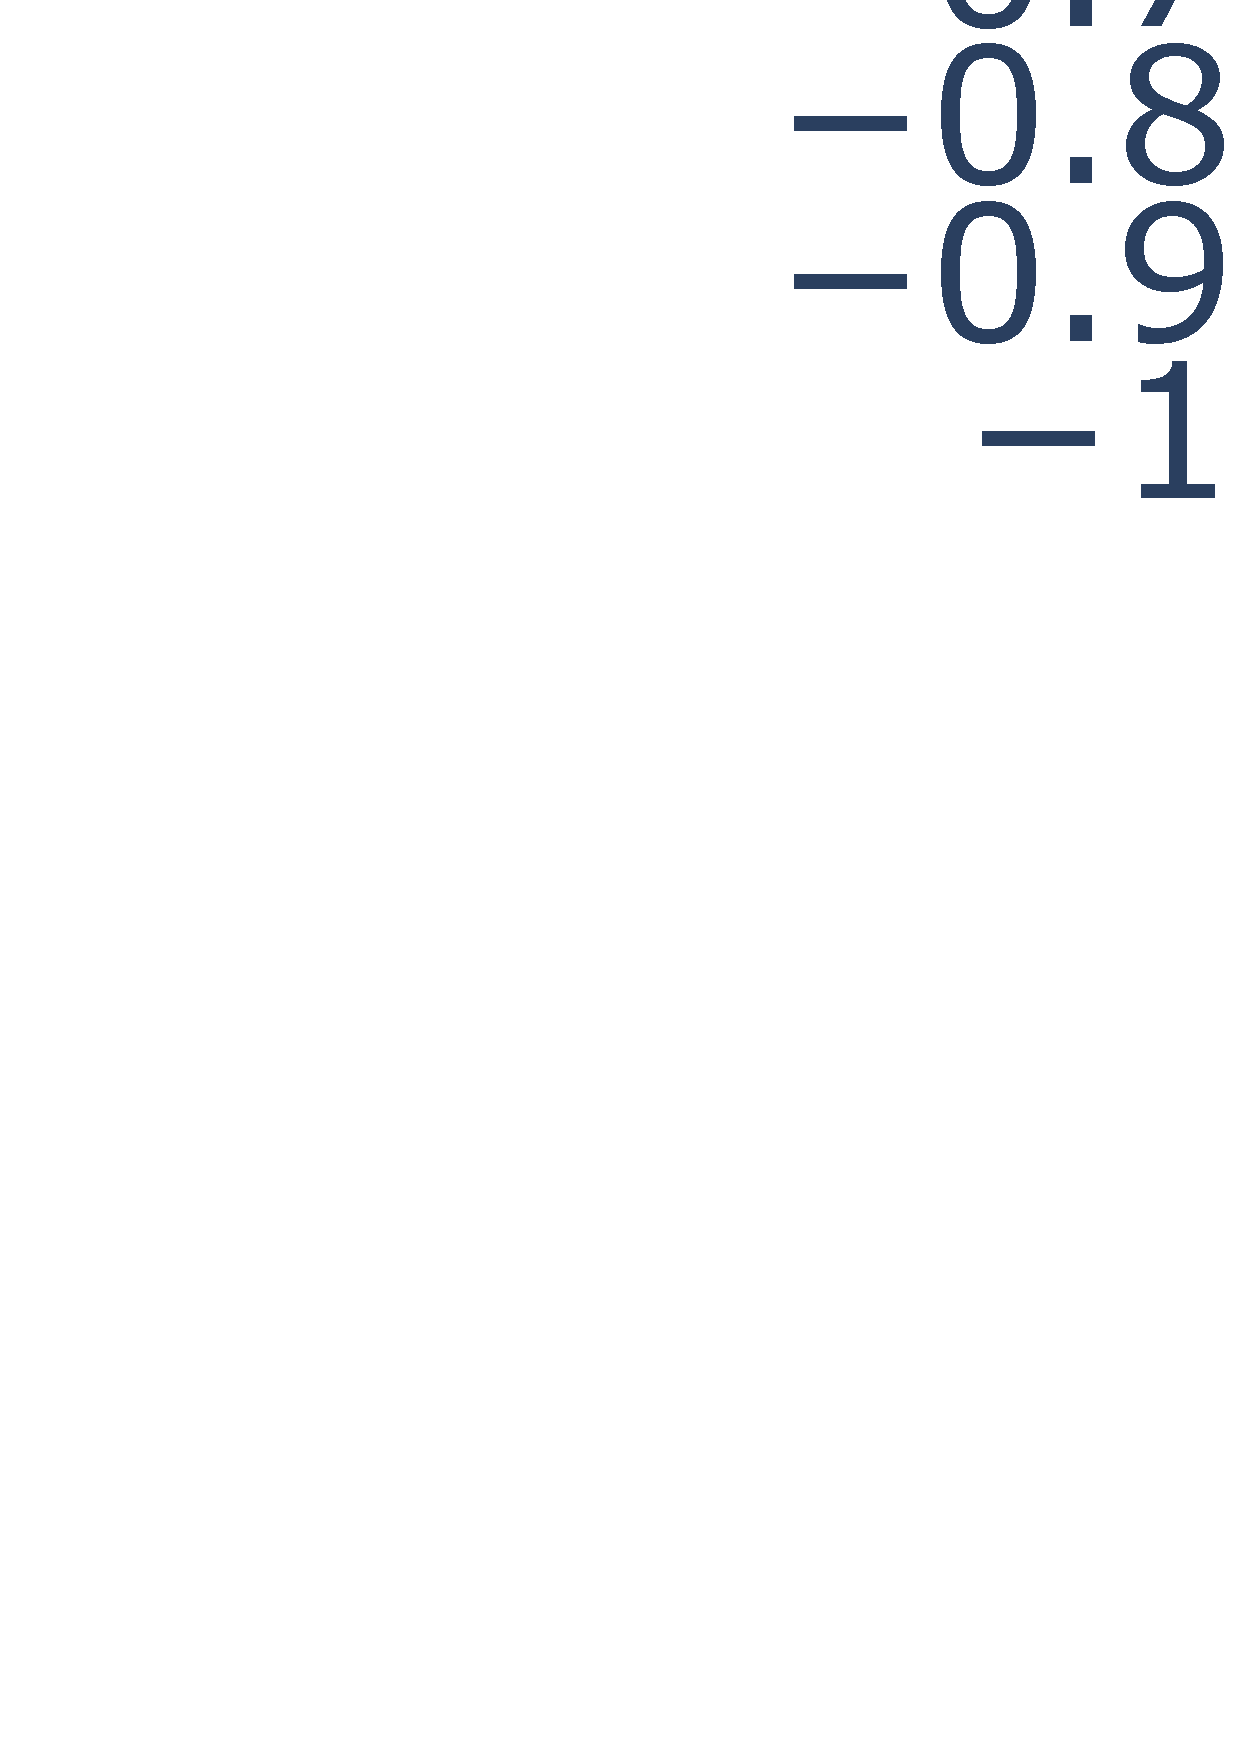
\includegraphics[width=0.8\linewidth]{images/01ContinuousVsDiscrete.pdf}
  %   \caption{Discrete samples (black points) from a continuous wave (grey line). Note that the amplitude is also truncated}
  %   \label{fig:ContinuousVsDiscrete}
  % \end{figure}
  
\section{Results}

\section{Discussion + Conclusion}

\section{References}

\end{document}
